\chapter*{Mathematical Bridge I: Linear Algebra for AI Thinking}
\addcontentsline{toc}{chapter}{Mathematical Bridge I: Linear Algebra for AI Thinking}

\begin{learninggoals}
\item Explain why AI work starts with a representation choice before it starts with a model choice.
\item Read vectors, matrices, dot products, and shapes as modeling statements rather than as isolated symbols.
\item Compute a weighted score by hand and explain what each term contributes.
\item Distinguish distance, similarity, and scale, and explain why they matter for downstream model behavior.
\item Interpret norms, linear maps, and projection as tools for controlling, comparing, and fitting representations.
\item Produce a one-page representation card before reporting that a model family is suitable for a task.
\end{learninggoals}

\begin{whychaptermatters}
This bridge makes the book's first modeling habit explicit: every example is already a representation choice. After reading it, students should be able to narrate rows, columns, shapes, and weighted sums in plain language instead of treating them as notation cleanup. The representation card becomes the math-side precursor to the baseline-design work in Chapter 4.
\end{whychaptermatters}

\begin{prereqbridge}
Use this as just-in-time review: read it now if linear-algebra notation feels rusty, or return when later chapters start leaning on vectors, matrices, and geometry. Comfort with high-school algebra is enough: variables, substitution, and evaluating expressions. Calculus is not required. Familiarity with Python lists or arrays is helpful but not required. Students who have already taken a linear algebra course should still skim because the AI-specific vocabulary here (representation, coordinate, weighted evidence) will recur throughout the book.
\end{prereqbridge}

Many students first meet linear algebra as a list of operations: add vectors, multiply matrices, solve systems. That is not the most helpful entry point for AI. In AI, linear algebra is the language that makes representations visible. It tells us what counts as one example, what counts as one coordinate, how many examples are being processed at once, what a score really is, and what kinds of similarity or geometry a method is quietly assuming.

The point here is not to re-teach every theorem from a full linear algebra course. The point is to make the objects in later chapters feel readable. If you can look at a vector or matrix and ask, ``what real thing does each row, column, or coordinate mean here?'' then the mathematics is already doing its job.

\begin{problemsolvinglens}
Before asking which model family to use, ask how one case is represented, what each coordinate means, what counts as similarity, and what a weighted combination of the coordinates would mean in plain language.
\end{problemsolvinglens}

\begin{thinkingtool}
\textbf{Representation audit.} Before blaming or praising a model, ask four questions: what counts as one example, what each coordinate means, what information has already been discarded, and what notion of similarity the representation makes easy.
\end{thinkingtool}

One compact summary holds the chapter together: a short \emph{representation card} that names what counts as one example, what the coordinates mean, what geometry matters, and what a linear score would mean in plain language.

\section*{Opening Case: One Student, One Email, One Image Patch}

Suppose we want to support three different AI tasks:

\begin{itemize}[leftmargin=*]
\item detect which students may need early human outreach,
\item estimate whether an email is spam,
\item estimate how many animals appear in a small aerial image crop.
\end{itemize}

These tasks look different on the surface, but they share one structural step. Each task needs a way to turn one case into a mathematical object that a model can read. A student becomes a list of measurements. An email becomes word counts, sender cues, or contextual embeddings. An image crop becomes pixel intensities or learned feature maps.

That is the first linear-algebra lesson of the book. AI does not begin with magic. It begins with a decision about representation.

\begin{center}
\small
\begin{tabular}{p{2.33cm}p{7.62cm}}
\toprule
Task & One possible machine-readable description \\
\midrule
Student support & Attendance rate, quiz average, missing assignments, and recent platform activity \\
Spam filtering & Counts of important words, sender reputation cues, link patterns, and message length \\
Image counting & Pixel values or local visual features extracted from a small patch \\
\bottomrule
\end{tabular}

\medskip
\noindent\textbf{Three tasks, one shared question.} What counts as one example, and what mathematical object will stand in for it?
\end{center}

\section*{Vectors Are Organized Descriptions}

A vector is an ordered collection of coordinates. In AI language, a vector is often just one represented example.

For the student-support task, we might record four normalized quantities for one student:
\[
x =
\begin{bmatrix}
0.92 \\
0.80 \\
0.10 \\
0.35
\end{bmatrix}
\]
where the coordinates mean:
\begin{itemize}[leftmargin=*]
\item \(0.92\): attendance rate,
\item \(0.80\): quiz average,
\item \(0.10\): fraction of assignments missed,
\item \(0.35\): recent platform inactivity score.
\end{itemize}

The notation matters less than the interpretation. The vector is not just ``four numbers.'' It is one student expressed through four chosen coordinates. Another representation choice would give a different vector and therefore a different modeling problem.

\begin{prereqbridge}
Read \(x_j\) as ``the \(j\)-th coordinate of the represented example.'' If the notation feels formal, translate it immediately back into the task language: attendance, quiz average, missed assignments, or inactivity.
\end{prereqbridge}

Two practical habits begin here.

First, order matters. Once the first coordinate means attendance and the second means quiz average, we cannot silently swap them later.

Second, scale matters. A coordinate measured from \(0\) to \(1000\) behaves differently from one measured from \(0\) to \(1\). Later chapters on nearest neighbors, regularization, and optimization all depend on this simple point.

\section*{Shapes, Batches, and Why Dimension Errors Matter}

A vector has a shape. A dataset has a shape. A batch of images or sequences has a shape. Shape is not bookkeeping. Shape states what counts as one case, what counts as one feature family, and what gets processed together. Misreading shape is one of the most common sources of silent bugs in AI work.

Consider three objects that appear across later chapters.

\textbf{One tabular row.} A single student described by four features is a vector $x \in \mathbb{R}^4$. In array-style notation, its shape is often written as $(4,)$: four numbers, one case.

\textbf{A bag-of-words batch.} Suppose we process $32$ emails at once, each represented as a count vector over a vocabulary of $10{,}000$ words. The batch is a matrix of shape $(32, 10000)$: $32$ rows for $32$ cases, $10{,}000$ columns for $10{,}000$ features.

\textbf{A token-by-token embedding sequence.} A sentence tokenized into $T$ tokens, where each token is embedded into $d$ dimensions, forms a matrix of shape $(T, d)$. Here the rows are positions in time or sequence, not independent cases. Transposing would swap that meaning and break any downstream operation that assumes the row is a token position.

\begin{prereqbridge}
In the mathematics of this book, vectors are usually written as column objects. In array libraries such as NumPy, a one-dimensional object with shape $(4,)$ is often treated as neither an explicit row nor an explicit column until it is reshaped. That software convention is convenient, but it can hide orientation mistakes. When matrix multiplication is the topic, it is safer to keep asking whether the object is being used as one column of features, one row of a dataset, or a library-level one-dimensional array.
\end{prereqbridge}

\begin{table}[t]
\centering
\small
\setlength{\tabcolsep}{4pt}
\begin{tabular}{p{2.72cm}p{2.38cm}p{4.85cm}}
\toprule
Object & Shape & What the dimensions mean \\
\midrule
Student feature vector & $(d,)$ & $d$ features for one student \\
Tabular dataset matrix & $(n, d)$ & $n$ examples, each with $d$ features \\
Bag-of-words batch & $(B, V)$ & $B$ documents in the batch, vocabulary size $V$ \\
Token embedding sequence & $(T, d)$ & $T$ token positions, each with a $d$-dim embedding \\
\bottomrule
\end{tabular}
\caption{Shape is a modeling statement. Rows and columns have different jobs, and confusing them causes dimension errors that are easy to miss in silent failure modes.}
\label{tab:shape-meanings}
\end{table}

A useful mini-checklist before writing any matrix operation:
\begin{itemize}[leftmargin=*]
\item What are the rows? (examples? positions? channels?)
\item What are the columns? (features? vocabulary items? time steps?)
\item What is repeated across the batch? (independent cases or steps of the same sequence?)
\item What would break if the object were transposed?
\end{itemize}

\begin{failurebox}
Dimension errors often succeed silently in Python. If a dot product or matrix multiply happens to have compatible shapes because an accidental transpose happens to work numerically, the model will train without error messages but learn from the wrong relationship. Checking what the dimensions mean before the operation---not just checking that the numbers multiply---is how practitioners catch this class of bug.
\end{failurebox}

\section*{Dot Products Are Weighted Evidence}

Once an example is represented as a vector, the simplest serious model asks a clean question: how much evidence does each coordinate contribute to one score?

That is the job of the dot product. If a weight vector is
\[
w =
\begin{bmatrix}
-1.6 \\
-1.1 \\
2.4 \\
1.8
\end{bmatrix},
\]
then the score \(w^\top x\) is
\[
w^\top x = (-1.6)(0.92) + (-1.1)(0.80) + (2.4)(0.10) + (1.8)(0.35).
\]
Working it out term by term gives
\[
w^\top x = -1.472 - 0.880 + 0.240 + 0.630 = -1.482.
\]

The point of this arithmetic is not the final decimal. The point is the interpretation.

\begin{itemize}[leftmargin=*]
\item Good attendance pushes the score down because its weight is negative.
\item Strong quiz performance also pushes the score down.
\item Missing assignments pushes the score up.
\item Inactivity also pushes the score up.
\end{itemize}

In other words, the dot product is a weighted evidence summary.

\begin{center}
\small
\begin{tabular}{p{2.73cm}p{1.82cm}p{1.82cm}p{2.73cm}}
\toprule
Coordinate & Value & Weight & Contribution \\
\midrule
Attendance & \(0.92\) & \(-1.6\) & \(-1.472\) \\
Quiz average & \(0.80\) & \(-1.1\) & \(-0.880\) \\
Assignments missed & \(0.10\) & \(2.4\) & \(0.240\) \\
Inactivity score & \(0.35\) & \(1.8\) & \(0.630\) \\
\bottomrule
\end{tabular}

\medskip
\noindent\textbf{Reading rule.} Multiply each coordinate by how much it matters, then add the contributions.
\end{center}

\begin{mathlens}
\textbf{Why the dot product appears everywhere.} A dot product is a weighted sum, and weighted sums are the simplest way to combine many weak signals into one score. Linear regression, logistic regression, attention scores, nearest-prototype methods, and many neural-network layers all reuse this structure. The later models are richer, but the weighted-sum idea never really leaves.
\end{mathlens}

\section*{From One Example to Many: Matrices As Datasets}

Once there is more than one example, it is wasteful to write every case separately. A matrix packages many vectors together.

Suppose three students are represented as rows:
\[
X =
\begin{bmatrix}
0.92 & 0.80 & 0.10 & 0.35 \\
0.70 & 0.62 & 0.30 & 0.55 \\
0.98 & 0.91 & 0.00 & 0.10
\end{bmatrix}.
\]

This matrix has shape \(3 \times 4\): three rows, four columns. In the dataset view:

\begin{itemize}[leftmargin=*]
\item rows are examples,
\item columns are features,
\item shape records how many cases and features are present.
\end{itemize}

This is one of the most useful sanity checks in practical ML. If a student thinks a dataset has \(n\) examples and \(d\) features, then the design matrix should have \(n\) rows and \(d\) columns. Many beginner bugs are simply shape misunderstandings wearing fancy clothes.

Matrix multiplication then applies one scoring rule to every row at once:
\[
Xw =
\begin{bmatrix}
0.92 & 0.80 & 0.10 & 0.35 \\
0.70 & 0.62 & 0.30 & 0.55 \\
0.98 & 0.91 & 0.00 & 0.10
\end{bmatrix}
\begin{bmatrix}
-1.6 \\
-1.1 \\
2.4 \\
1.8
\end{bmatrix}
=
\begin{bmatrix}
-1.482 \\
-0.092 \\
-2.389
\end{bmatrix}.
\]

Now the same weighted rule has produced one score for each student.

\begin{mathlens}
If the rows of \(X\) are examples \(x_1^\top,\ldots,x_n^\top\), then
\[
Xw=
\begin{bmatrix}
x_1^\top w\\
x_2^\top w\\
\vdots\\
x_n^\top w
\end{bmatrix}.
\]
So matrix-vector multiplication is just repeated dot products, one row at a time. The matrix is not doing a different kind of math; it is packaging the same linear rule so it can be applied to many examples at once.
\end{mathlens}

\begin{codeexample}
def linear_scores(X, w, b=0.0):
    scores = []
    for row in X:
        if len(row) != len(w):
            raise ValueError("row and weight vector must have the same length")
        score = b
        for value, weight in zip(row, w):
            score += value * weight
        scores.append(score)
    return scores
\end{codeexample}

The point of this tiny function is not software convenience. It is to make the mechanism visible. A matrix is not mystical. It is a compact way to store many represented cases, and matrix multiplication applies one structured computation to every row.

\begin{example}[Matrix-Vector Product by Hand]
Consider three students, each described by two features: attendance rate and number of late submissions. The design matrix and weight vector are

\[
X =
\begin{bmatrix}
0.90 & 1 \\
0.60 & 4 \\
0.80 & 0
\end{bmatrix},
\qquad
w =
\begin{bmatrix}
-1.5 \\
2.0
\end{bmatrix}.
\]

The columns mean: first column = attendance rate, second column = number of late submissions. The weights say: good attendance lowers the risk score (\(-1.5\)), while late submissions raise it (\(+2.0\)).

Computing \(Xw\) row by row:

\begin{itemize}[leftmargin=*]
\item \textbf{Student 1:} \((-1.5)(0.90) + (2.0)(1) = -1.35 + 2.0 = 0.65\)
\item \textbf{Student 2:} \((-1.5)(0.60) + (2.0)(4) = -0.90 + 8.0 = 7.10\)
\item \textbf{Student 3:} \((-1.5)(0.80) + (2.0)(0) = -1.20 + 0.0 = -1.20\)
\end{itemize}

\[
Xw =
\begin{bmatrix}
0.65 \\
7.10 \\
-1.20
\end{bmatrix}.
\]

Under this weighted rule, Student 2 receives the largest score, Student 1 an intermediate score, and Student 3 the smallest score. That ordering reflects how strongly late submissions outweigh attendance in the chosen weights. A later chapter may turn such scores into risk categories or actions, but at this stage the safe claim is the ranking induced by the linear rule, not a final decision label.

This is the key idea: the same weight vector \(w\) is applied to every row simultaneously. The matrix does not change the structure of the computation---it only packages it so every student gets scored in one operation.
\end{example}

\section*{Sparse, Dense, and Missingness as Representation Facts}

Representations are not only numeric. They differ in density, noise, and missingness, and those differences change how models behave.

A \emph{sparse} representation has many zero coordinates. A bag-of-words vector for one email drawn from a vocabulary of $50{,}000$ words will usually have fewer than $200$ nonzero entries. Most words in the vocabulary simply do not appear in that message. Sparsity is not a deficiency of the representation. It is information: a coordinate being zero means the corresponding feature is absent.

A \emph{dense} representation has very few zeros. A learned word embedding of dimension $300$ will typically have all $300$ coordinates populated with small but nonzero values. Dense representations are compact and support smooth geometric operations like cosine similarity, but they offer no inherent interpretability for individual coordinates.

A \emph{partially observed} representation has coordinates that are missing for structural reasons, not random ones. A student record may have quiz scores for seven of ten weeks because a student joined late. A sensor trace may be missing every other reading because the device transmits on an alternating schedule. In each case, the absence of a value carries information about the process that generated the data.

\begin{table}[t]
\centering
\small
\setlength{\tabcolsep}{4pt}
\begin{tabular}{p{1.89cm}p{3.26cm}p{4.8cm}}
\toprule
Type & Example & What absence means \\
\midrule
Sparse & Bag-of-words email vector & Word did not appear in this message \\
Dense & Learned word embedding & Most coordinates are nonzero; zero does not mean ``feature absent'' \\
Partially observed & Student engagement record with gaps & Student may not have been enrolled yet, or event did not fire \\
\bottomrule
\end{tabular}
\caption{Representation quality includes density, which coordinates are absent, and whether absence is informative. A recorded zero, a structurally missing entry, and an unknown value are different representational states that may need different handling.}
\label{tab:sparse-dense-missing}
\end{table}

Three practical lessons follow.

\emph{Sparse representations support fast inner products but can break distance-based methods.} Euclidean distance is driven by coordinates where the two vectors differ. In very sparse vectors, that often means a small number of mismatched nonzero entries dominate the distance, while the many shared zeros contribute little. Cosine similarity can handle this better in some cases, but neither operation treats ``both missing this word'' and ``both present on this word'' as the same kind of evidence.

\emph{Dense embeddings lose interpretability at the coordinate level.} A single coordinate of a word embedding does not mean anything human-readable. The space as a whole may encode meaning geometrically, but the coordinates individually do not.

\emph{Missingness in tabular data is often not random.} Imputing a missing value with a mean or zero can be useful, but only after we ask what the missingness means and whether it should be represented explicitly with a mask or indicator. If the value is missing because the student dropped before week eight, or because a sensor was offline after a power failure, blindly replacing it with one default number can inject the wrong kind of signal. Later chapters on reliability and deployment return to this point. For now, the lesson is that ``missing'' is not automatically the same thing as zero; it is part of the representation and data-generation story.

\section*{Geometry: Distance, Similarity, and Scale}

Once cases live in vectors, geometry starts to matter. The geometry is not a picture drawn after the fact. It is part of the model.

If two represented students are
\[
x =
\begin{bmatrix}
0.92 \\
0.80 \\
0.10 \\
0.35
\end{bmatrix},
\qquad
z =
\begin{bmatrix}
0.88 \\
0.78 \\
0.12 \\
0.40
\end{bmatrix},
\]
their Euclidean distance is
\begin{align*}
\|x-z\|_2 &= \bigl[(0.92{-}0.88)^2 + (0.80{-}0.78)^2 \\
&\quad\;+ (0.10{-}0.12)^2 + (0.35{-}0.40)^2\bigr]^{1/2}.
\end{align*}
This distance is small, so the two cases are close under that geometry.

Cosine similarity asks a different question. Instead of asking whether the vectors are close in absolute position, it asks whether they point in nearly the same direction:
\[
\cos(\theta) = \frac{x^\top z}{\|x\|_2 \|z\|_2}.
\]
This is useful when overall scale should matter less than pattern. In language or embedding-style problems, two long vectors can represent similar meaning even if one is globally larger than the other.

\begin{failurebox}
Distance-based methods can fail for a boring reason: one coordinate dominates because it is measured on a much larger numeric scale. If age is stored in years but income is stored in dollars, then raw Euclidean distance mostly measures income. That is not a property of the world. It is a property of the chosen units. The first recovery move is usually to put the coordinates on comparable scales before trusting the geometry.
\end{failurebox}

\section*{Norms, Size, and Regularization Intuition}

A norm measures the size of a vector. Two common norms are
\[
\|w\|_1 = \sum_{j=1}^{d} |w_j|,
\qquad
\|w\|_2 = \sqrt{\sum_{j=1}^{d} w_j^2}.
\]

Later chapters use these ideas for regularization. The reason is simple, but it depends on the representation being fixed. Once features have been put on a defended scale, a model with very large coefficients can become brittle, overly reactive, or too willing to fit accidental quirks in the training data. Penalizing coefficient size is one way of expressing a preference for simpler behavior unless the data strongly demands otherwise.

Students should not hear the word \emph{regularization} and think only ``extra term in the objective.'' The modeling question is more useful:

\begin{quote}
How much coefficient size, complexity, or sensitivity are we willing to tolerate before we think the fit has become unstable?
\end{quote}

\section*{Linear Maps, Projections, and Fitting}

A linear map is a rule that transforms one vector into another while preserving weighted-sum structure. In AI terms, it is a structured feature transformation.

This matters because many models do not work directly on the raw input. They work on transformed coordinates. Even when later chapters discuss embeddings or learned internal layers, one recurring question survives:

\begin{quote}
What transformation is making the relevant structure easier to see?
\end{quote}

Projection is the cleanest first fitting intuition. Suppose the world is more complicated than the model class we have allowed. Then training is often not finding the truth exactly. It is finding the closest allowed approximation under a chosen notion of error.

That is the useful least-squares picture. A linear model does not win because it captures every detail of reality. It wins when the best projection into the linear family is already good enough for the task.

\begin{mathlens}
For the simplest projection onto a one-dimensional direction \(u\) with \(\|u\|_2=1\), the fitted point is
\[
\hat{x}=(x^\top u)u.
\]
The residual is \(r=x-\hat{x}\). The key geometric fact is
\[
r^\top u=0,
\]
so the leftover error is orthogonal to the direction we kept. In least squares, this is the meaning of ``best fit'': after projection, no remaining error points along the allowed direction.
\end{mathlens}

\begin{mathlens}
A projection map is itself a linear map. If \(u\) is a unit direction, then
\[
P_u(x)=(u^\top x)u
\]
keeps only the component of \(x\) that lies along \(u\). Applying it twice changes nothing:
\[
P_u(P_u(x))=P_u(x).
\]
That is the algebraic version of geometric fitting: once a vector has been projected onto the allowed line, projecting again cannot improve it further.
\end{mathlens}

\begin{advancednote}
Students often hear that linear models are ``simple'' and stop there. A better statement is that linear models define a restricted hypothesis class with very transparent geometry. That restriction is sometimes a weakness, but it is also what makes the class interpretable, diagnosable, and often surprisingly competitive.
\end{advancednote}

\begin{example}[Projection in One Dimension]
Suppose we observe three data points \(y = [2, 4, 6]\) and we want to fit a constant model---a single number \(c\) that stands in for all three values. Which constant is best?

The mean is \(\bar{y} = (2 + 4 + 6)/3 = 4\). The residuals from the mean are
\[
r = [2 - 4,\; 4 - 4,\; 6 - 4] = [-2,\; 0,\; 2].
\]
The sum of squared residuals is
\[
SS(\bar{y}) = (-2)^2 + 0^2 + 2^2 = 4 + 0 + 4 = 8.
\]

Now try a different constant, say \(c = 3\):
\[
r = [2-3,\; 4-3,\; 6-3] = [-1,\; 1,\; 3].
\]
\[
SS(3) = (-1)^2 + 1^2 + 3^2 = 1 + 1 + 9 = 11.
\]

The sum of squares rose from \(8\) to \(11\) when we moved away from the mean. Any other constant will produce a sum of squares no smaller than \(8\). In coefficient terms, the best constant is \(4\). In geometric terms, the data vector \([2,4,6]\) projects onto the constant-model class as \([4,4,4]\), the unique member of that class that sits closest to the data under squared error.

This is the geometry of least-squares fitting in miniature. The model class (all constant functions) is a restricted family. Training finds the member of that family that is closest to the target values. The residuals \([-2, 0, 2]\) are orthogonal to the constant direction---they average to zero, meaning no constant shift can reduce the error further.
\end{example}

\section*{Linear Separability and What a Hyperplane Can Actually Express}

A linear score $w^\top x + b$ divides the input space into two half-spaces: examples where the score is positive and examples where it is negative. In two dimensions, that boundary is a line. In three dimensions, it is a plane. In $d$ dimensions, it is a hyperplane.

Understanding what a hyperplane can and cannot separate gives a concrete reason for why later chapters need trees, kernels, and neural nonlinearities. Without this picture, ``nonlinearity matters'' can sound like folklore. With it, the limitation becomes a specific geometric fact.

\textbf{A case where a line succeeds.} Consider four points in two dimensions:
\[
(1,1),\ (1,2),\ (3,3),\ (4,4).
\]
Suppose the first two are class A and the last two are class B. A line such as $x_1 + x_2 = 5$ separates them cleanly. Here the linear model is sufficient.

\textbf{A case where a line fails: the XOR pattern.} Now consider four points:
\[
(0,0),\ (1,1),\ (1,0),\ (0,1).
\]
Suppose $(0,0)$ and $(1,1)$ are class A, and $(1,0)$ and $(0,1)$ are class B. Any line through this plane will put at least one point on the wrong side. There is no linear decision boundary that correctly separates these four points.

\begin{figure}[t]
\centering
\resizebox{\linewidth}{!}{%
\begin{tikzpicture}[font=\small, x=2.0cm, y=2.0cm]
\begin{scope}
\draw[->] (-0.2,0) -- (1.8,0) node[right] {$x_1$};
\draw[->] (0,-0.2) -- (0,1.8) node[above] {$x_2$};
\filldraw (0.3,0.4) circle (2pt) node[above right] {A};
\filldraw (0.4,1.2) circle (2pt) node[above right] {A};
\draw (1.2,0.8) circle (2pt) node[above right] {B};
\draw (1.5,1.5) circle (2pt) node[above right] {B};
\draw[thick, dashed] (0.6,1.8) -- (1.8,0.0);
\node at (0.9,-0.35) {separable};
\end{scope}
\begin{scope}[xshift=5.2cm]
\draw[->] (-0.2,0) -- (1.8,0) node[right] {$x_1$};
\draw[->] (0,-0.2) -- (0,1.8) node[above] {$x_2$};
\filldraw (0.0,0.0) circle (2pt) node[above right] {A};
\filldraw (1.0,1.0) circle (2pt) node[above right] {A};
\draw (1.0,0.0) circle (2pt) node[above right] {B};
\draw (0.0,1.0) circle (2pt) node[above right] {B};
\node at (0.5,-0.35) {not separable (XOR)};
\end{scope}
\end{tikzpicture}%
}
\caption{Left: a line separates the two classes. Right: the XOR pattern cannot be separated by any line. The filled points are class A; the open points are class B.}
\label{fig:linear-separability}
\end{figure}

The XOR pattern is not a contrived puzzle. It represents the general situation where the decision depends on an \emph{interaction} between features: being at position $(0,0)$ and being at position $(1,1)$ belong to the same class not because of either coordinate alone, but because of the combination. A linear model working on raw coordinates cannot represent that.

This is the geometric reason why interaction features, kernel methods, tree splits, and neural nonlinearities matter. Each one extends the expressible boundary beyond the flat hyperplane. Trees do it by recursive axis-aligned cuts. Kernel methods do it by implicitly working in a richer feature space. Neural networks do it by composing nonlinear transformations.

\begin{advancednote}
The formal study of which problems linear models can solve is part of the theory of VC dimension and linear dichotomies. For this book, the geometric picture is enough: a hyperplane is a powerful tool when the relevant decision boundary is roughly flat in the feature space, and a poor tool when the boundary requires reasoning about feature interactions.
\end{advancednote}

\section*{Low-Dimensional Structure}

Real datasets often have many coordinates but fewer truly important directions. In image, language, and tabular problems alike, some features overlap, some move together, and some mostly repeat what others already say.

The practical lesson is not that every dataset can be compressed aggressively. The lesson is that high ambient dimension does not always mean high effective complexity. This intuition later supports PCA, embeddings, representation learning, and transfer learning.

For a tabular example, imagine four recorded features: attendance, quiz average, assignment completion, and recent platform activity. Those are four coordinates, but they may not vary independently. Students who attend regularly may also submit more work and stay active on the platform, so much of the variation may lie near one broader ``overall engagement'' direction. The raw representation is four-dimensional, but the dominant structure may live in only one or two directions.

\begin{figure}[t]
\centering
\definecolor{b1dirBlue}{RGB}{56,103,170}
\definecolor{b1ptOrange}{RGB}{197,111,43}
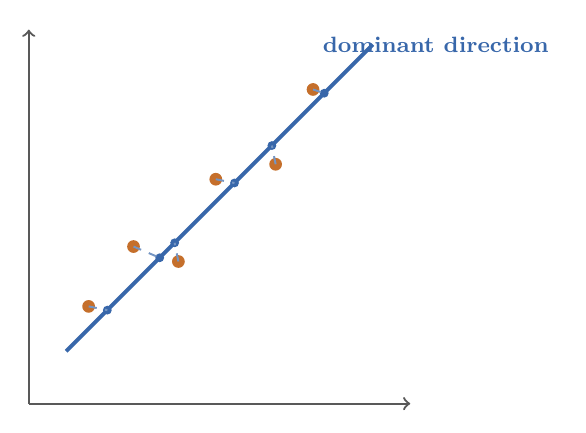
\begin{tikzpicture}[x=0.95cm,y=0.95cm,font=\small]
  \draw[->, line width=0.8pt, black!65] (0.2,0.2) -- (5.3,0.2);
  \draw[->, line width=0.8pt, black!65] (0.2,0.2) -- (0.2,5.2);

  \draw[b1dirBlue, line width=1.4pt] (0.7,0.9) -- (4.8,5.0);
  \node[anchor=west, text=b1dirBlue, font=\footnotesize\bfseries] at (4.0,5.0)
    {dominant direction};

  \foreach \px/\py/\qx/\qy in {
    1.0/1.5/1.25/1.45,
    1.6/2.3/1.95/2.15,
    2.2/2.1/2.15/2.35,
    2.7/3.2/2.95/3.15,
    3.5/3.4/3.45/3.65,
    4.0/4.4/4.15/4.35
  }{
    \fill[b1ptOrange] (\px,\py) circle (2.3pt);
    \fill[b1dirBlue] (\qx,\qy) circle (1.6pt);
    \draw[b1dirBlue!70, dashed, line width=0.7pt] (\px,\py) -- (\qx,\qy);
  }
\end{tikzpicture}
\caption{Several visible coordinates can still lie near one dominant direction. Projection keeps the variation along that direction and discards the smaller residual deviations away from it.}
\label{fig:bridge-lowdim-projection}
\end{figure}

Figure~\ref{fig:bridge-lowdim-projection} shows the basic geometry. The original points live in a two-coordinate display, but most of their variation is organized by one shared diagonal trend and only a small residual remains off that line.

\begin{mathlens}
A projection onto a lower-dimensional subspace keeps only a smaller set of allowed directions. If \(u_1,\ldots,u_k\) are orthonormal directions, then the projection of \(x\) onto their span is
\[
 \hat{x}=\sum_{j=1}^{k}(u_j^\top x)u_j.
\]
Each coefficient \(u_j^\top x\) tells us how much of \(x\) lies along one kept direction. If \(k \ll d\), then the approximation uses far fewer directions than the raw coordinate count. The discarded residual \(r=x-\hat{x}\) is orthogonal to every kept direction, so the kept subspace captures the part of the vector that those directions can explain.
\end{mathlens}

Students do not need a full singular-value-decomposition treatment here. They do need the idea that useful structure can live in fewer directions than the raw coordinate count suggests.

\section*{Chapter Artifact: Representation Card}

\begin{quote}
\noindent\textbf{Representation Card}

\medskip
\begin{tabular}{>{\raggedright\arraybackslash}p{2.6cm}>{\raggedright\arraybackslash}p{5.4cm}}
\toprule
Field & What to write \\
\midrule
One example is... & Name the basic case: one student, one email, one image patch, one customer session, one hour of sensor data \\
Coordinates are... & Name each feature family and what each coordinate means \\
What is lost? & State what the representation throws away or blurs \\
What geometry matters? & Distance, angle, overlap, ordering, or something else \\
What does a linear score mean? & Explain what a weighted sum would count as evidence for or against \\
Main representation risk & State the most likely mismatch between representation and task \\
\bottomrule
\end{tabular}
\end{quote}

If this card cannot be written clearly, later model debates are usually premature.

\section*{Common Mistakes}

\begin{mistakebox}
\item \textbf{Treating a vector as just a bag of numbers.} A vector is a chosen representation, not a random pile of values.
\item \textbf{Confusing row count with feature count.} One case and one feature family play different roles in a dataset.
\item \textbf{Ignoring scale when distance or nearest neighbors matter.} Geometry depends on units.
\item \textbf{Treating a large dot product as self-explanatory.} A weighted sum only matters relative to the chosen representation.
\item \textbf{Thinking that more dimensions automatically mean more useful information.} Extra coordinates can just as easily add noise or redundancy.
\end{mistakebox}

\section*{Looking Ahead}

The geometric language of representation is now in place: vectors, matrices, weighted scores, distance, and projection. The next bridge adds the uncertainty language that makes those scores trainable and interpretable: probability, loss, empirical risk, and gradient signals. Together they prepare the main text, where Chapter 1 turns those mathematical objects into a defensible learning problem.

The representation card from this bridge becomes the starting document for the learning-signal card in the next bridge and later for the baseline-design work that begins in Chapter 4.

\begin{chaptersummary}
\item Linear algebra matters in AI because representation is already part of the model.
\item A vector is one represented case, and a matrix is many represented cases organized together.
\item A dot product is a weighted evidence summary.
\item Distance, similarity, and scale are modeling assumptions, not just visualization choices.
\item Norms measure size and later become regularization tools.
\item The main deliverable of the chapter is a representation card written before declaring that a model family is a good fit.
\end{chaptersummary}

\begin{studyquestions}
\item Why is representation choice already a modeling decision rather than a neutral preprocessing step?
\item In plain language, what does the dot product \(w^\top x\) mean in a decision-support problem?
\item Why can Euclidean distance and cosine similarity lead to different judgments about what counts as ``similar''?
\item What does it mean to say that fitting can be understood as projection into an allowed model class?
\end{studyquestions}

\begin{exercises}
\item Write a four-coordinate vector for a student-support problem and explain the meaning of each coordinate in one sentence.
\item For the vector \(x = [0.9, 0.7, 0.2]^\top\) and the weight vector \(w = [-2, 1, 3]^\top\), compute \(w^\top x\) and explain what each contribution means.
\item Construct a \(3 \times 4\) design matrix for three emails with four hand-chosen features. State clearly what the rows and columns represent.
\item Give one situation in which cosine similarity would be a better comparison than Euclidean distance, and one situation in which it would be worse.
\item Fill out a representation card for spam filtering, student support, or a simple image task. If you plan to carry one running case through the book, keep the same case and add one sentence saying which coordinates Chapter 1's framing memo would treat as acceptable inputs at prediction time.
\end{exercises}

\begin{challengeexercises}
\item Show with a tiny numeric example that rescaling one feature can change which case is the nearest neighbor, even when all other coordinates stay the same.
\item Give two different representations for the same task, explain what each preserves, and argue which one makes a linear score more meaningful.
\item Suppose a target cannot be expressed exactly by any weighted sum of the available features. Explain why least-squares fitting can still be read as finding the closest allowed predictor.
\end{challengeexercises}
